
\documentclass[a4paper,11pt,twoside,final]{scrreprt}


\usepackage{ngerman}  %Silbentrennung
\usepackage[T1]{fontenc} %Schriftenkodierung nach westeuropäischem Standard
%\usepackage[latin1]{inputenc}
\usepackage{lmodern}  %Anzeige auf Computerbildschirmen

\usepackage{% 
	ellipsis, % Korrigiert den Weißraum um Auslassungspunkte
	ragged2e, % Ermöglicht Flattersatz mit Silbentrennung
	marginnote,% Für bessere Randnotizen mit \marginnote statt
	% \marginline
}
\usepackage[tracking=true]{microtype}
\DeclareMicrotypeSet*[tracking]{my}% 
{ font = */*/*/sc/* }% 
\SetTracking{ encoding = *, shape = sc }{ 45 }% Hier wird festgelegt,
% dass alle Passagen in Kapitälchen automatisch leicht
% gesperrt werden. Das Paket soul, das ich früher empfohlen
% habe ist damit für diese Zwecke nicht mehr nötig.
%
%%%%%%%%%%%%% Verschiedene Schriften, die ich nutze:
% Es ist natürlich nicht sinnvoll mehrere Pakete zu
% laden, die immer wieder die Serifenschrift umstellen.
% Suchen Sie /eine/ aus und löschen Sie das erste
% Prozent-Zeichen in der Zeile A) oder B) oder ...  

\usepackage{graphicx}
\usepackage{epstopdf}


%\usepackage{eps}  % Um eps /jpeg/png parallel einzubinden

\begin{document}
	
\begin{titlepage}
    \begin{center}
        \vspace*{1cm}
        
        \Huge
        \textbf{Institute of Applied Mechanics}
		\textbf{Department of Fluid Mechanics}
        
        \vspace{0.5cm}
        \LARGE
        Technical University of Clausthal
        
        \vspace{2cm}
        
        %\includegraphics[width=0.4\textwidth]{university_logo} % Replace 'university_logo' with the actual filename of your university logo
        
        \vspace{2cm}
        
        
        
        \vspace{1cm}
        
        \textbf{\Huge Neural Network-based Detection of Taylor Vortices in Annular Flow Systems}
        
        \vfill

        \textbf{\LARGE Mahyar Alikhani}
        \vspace{1cm}

		\Large
        Supervisors:\\
		Prof. Dr.-Ing Andreas Rausch \\
		Prof. Dr.-Ing. Gunther Brenner \\
		M.Sc. Kathrin Susanne Skinder

        
        \vspace{0.8cm}
        
        \Large
        Date: \today % or put the specific date
        
    \end{center}
\end{titlepage}
	
\chapter{Bestandteile eines Exposes für wissenschaftliche Arbeiten }
\label{chap:Expose}
	
Ein Expose ist eine freiwillige Arbeit. Es dient der Vorbereitung einer wissenschaftlichen (Abschluss-)Arbeit
und dokumentiert dies. Der Student soll dabei die Aufgabenstellung reflektieren 
und sich in geeigneter Weise mit dem Stoff beschäftigen und in die Aufgabe einarbeiten.
Erfahrungsgemäß steigern gute Exposes die Qualität der späteren Arbeit und schlagen sich positiv in der Note
wieder. Dies liegt daran, dass die Studierenden ihre Aufgabe strukturierter angehen und besser organisiert sind. 
Eine realistische Zeitplanung hilft dabei und ist wichtiger Bestandteil. ein gutes Expose ist für den Betreuer 
gewissermaßen auch der Nachweis, dass der Student die Aufgabenstellung verstanden hat.

Dieses Dokument ist als Checkliste zu verstehen. Für die Strukturierung und Gliederung orientieren Sie sich 
bitte an anderen Abschlussarbeiten bzw. den üblichen Standards.

Folgende Elemente sind Bestandteil eines Exposes:

	\begin{description}
		\item[Problemstellung] \hfill \\  
		Hier wird ganz allgemein das Problem umrissen. In den Ingenieurwissenschaften werden in der Regel 
		technische Probleme gelöst, die aber auch eine gesellschaftliche Relevanz haben können. 
		Hier ist eine grundsätzliche Einführung in das Problem gefordert, die die Begründung für den 
		angestrebten Erkenntnisgewinn liefert.  Nach der Lektüre dieses Abschnitts muss dem Leser klar sein, 
		warum diese Arbeit verfasst wurde. Dieser Teil wird auch als Motivation bezeichnet.
		
		Beispielsweise ist die Teillastströmung einer Turbomaschine stark instationär und hoch turbulent.
		Das Resultat können schädigungsrelevante Anregungen der Maschine sein. Bei Verbrennungskraftmaschinen
		könnten etwa niedrige Wirkungsgrade oder das Emmissionsverhalten als Problem aufgefasst werden.
		Dies kann auch unter einem gesellschaftlichen Kontext betrachtet werden, aus dem heraus Handlungsbedarf 
		entsteht.
		Die Problemstellung ist häufig
		sehr allgemein formuliert und ist stets Bestandteil der Einleitung wissenschaftlicher Arbeiten.
	
		
		\item[Fragestellung - \textquotedblleft nach dem Leben, dem Universum und dem ganzen Rest\textquotedblright] \hfill \\ 
		 Damit eine Antwort, also die anzufertigenden wissenschaftlichen Arbeit, einen Nutzen hat, muss die 
		 Frage die am Anfang steht (oder stehen sollte), bekannt sein. 
		 Aus der Problemstellung ist eine, nun schon konkreter formulierte, Fragestellung abzuleiten.
		 Am Beispiel der genannten turbulenten Teillastströmung könnte die Frage lauten, inwiefern modizifierte  
		 Turbulenzmodelle Strömungen genauer wiedergeben können.
		 Eine Fragestellung wiederum führt auf die Aufgabenstellung, welche Arbeiten der Studierende 
		 zur Beantwortung der Fragestellung durchführen soll. Dabei ist je nach Anspruch der Arbeit der
		 Grad der eigenständigen Bearbeitung zu differenzieren.
		 \textquotedblleft Jetzt wo ich die Antwort kenne, hätte ich gerne meine Problem zurück.\textquotedblright
		 
		\item[Literatur]  \hfill \\ 
		Eine erste Literaturrecherche ist hier durchzuführen. Sie nimmt bereits einen Teil der eigentlichen Arbeit vorweg. Hier wird häufig Literatur zitiert, die die Problemstellung näher beschreibt oder es werden die Quellen	genannt, auf denen die Arbeit aufbaut. Zu den genannten Quellen gehört selbstverständlich auch 
		ein Literaturverzeichnis.
		
		\item[Theoretische Einbindung/Stand der Technik] \hfill \\ 
		Eine kurze Zusammenfassung, die den Stand der Technik wiedergibt. Der Literaturstand kann bereits bei der
		Problembeschreibung wiedergegeben werden, kann aber auch in einem eigenen Abschnitt behandelt werden. Eine detaillierte Fassung ist Bestandteil der späteren Arbeit.
		
		
		\item[Methodik/Vorgehensweise] \hfill \\ 
		Wie gedenken Sie die Fragestellung zu beantworten? Wie gehen Sie vor? Erste Hinweise hierfür liefert Ihnen
		in der Regel die Aufgabenstellung des Lehrstuhls, sofern diese schon vorliegt. Falls Ihr Thema nicht ausgeschrieben war, müssen Sie die Aufgabenstellung gemeinsam mit Ihrem Betreuer entwickeln.
		
		
		 
		\item[Zeitplan] \hfill \\
		Es empfiehlt sich Gantt-Diagramme zu nutzen. Hier stellen Balken über einer Zeitachse Dauer und Abhängigkeit von einzelnen Arbeitspaketen dar. Dieses Werkzeug wird im Projektmanagement verwendet und ist sehr hilfreich um eine realistische Zeitplanung aufzustellen.
		Dafür seien einige Dinge genannt, die Sie bedenken sollten: Wie viele Stunden arbeiten sie pro Woche? Haben Sie noch andere Vorlesungen? Planen Sie Prüfungen? Haben Sie Feiertage oder noch Prüfungen abzulegen?
		Haben Sie einen Nebenjob? Fragen Sie auch unbedingt Ihren Betreuer, ob er Ihren Zeitplan für machbar hält.
		

\begin{figure}
\centering
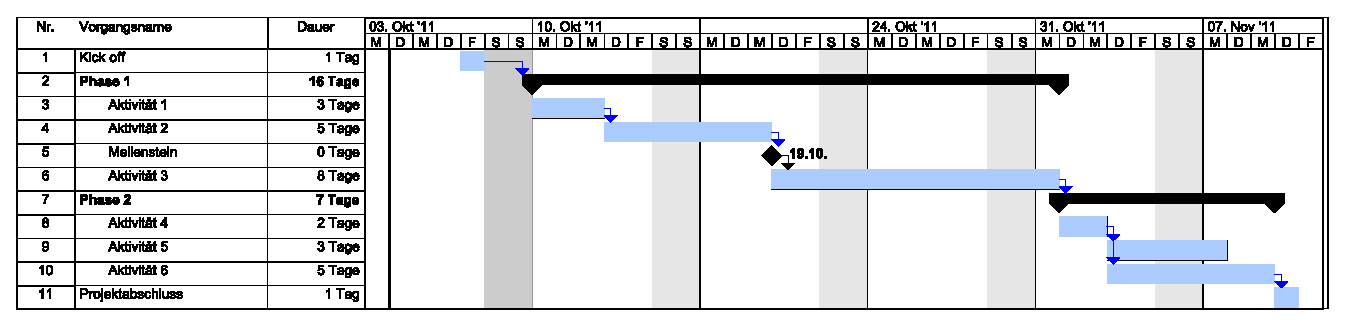
\includegraphics[width=\textwidth]{Gantt_diagramm}
\caption[Gantt-Diagramm]{Beispiel für ein Gantt-Diagramm}
\label{fig:Gantt_diagramm}
\end{figure}
  
		 
		  
		 
	\end{description}
	
	
\end{document}